\section{Theory}

\subsection{Analog circuit}
\label{sec:analogCircuit}
The analog circuit has input signals delivered by the digital circuitry, and delivers its output to two ADCs. The analog circuit diagram is given in figure \ref{fig:analogCircuit}, where each of the four pixel block has the circuit given in figure \ref{fig:pixelCircuit}.

\begin{figure}
    \centering
    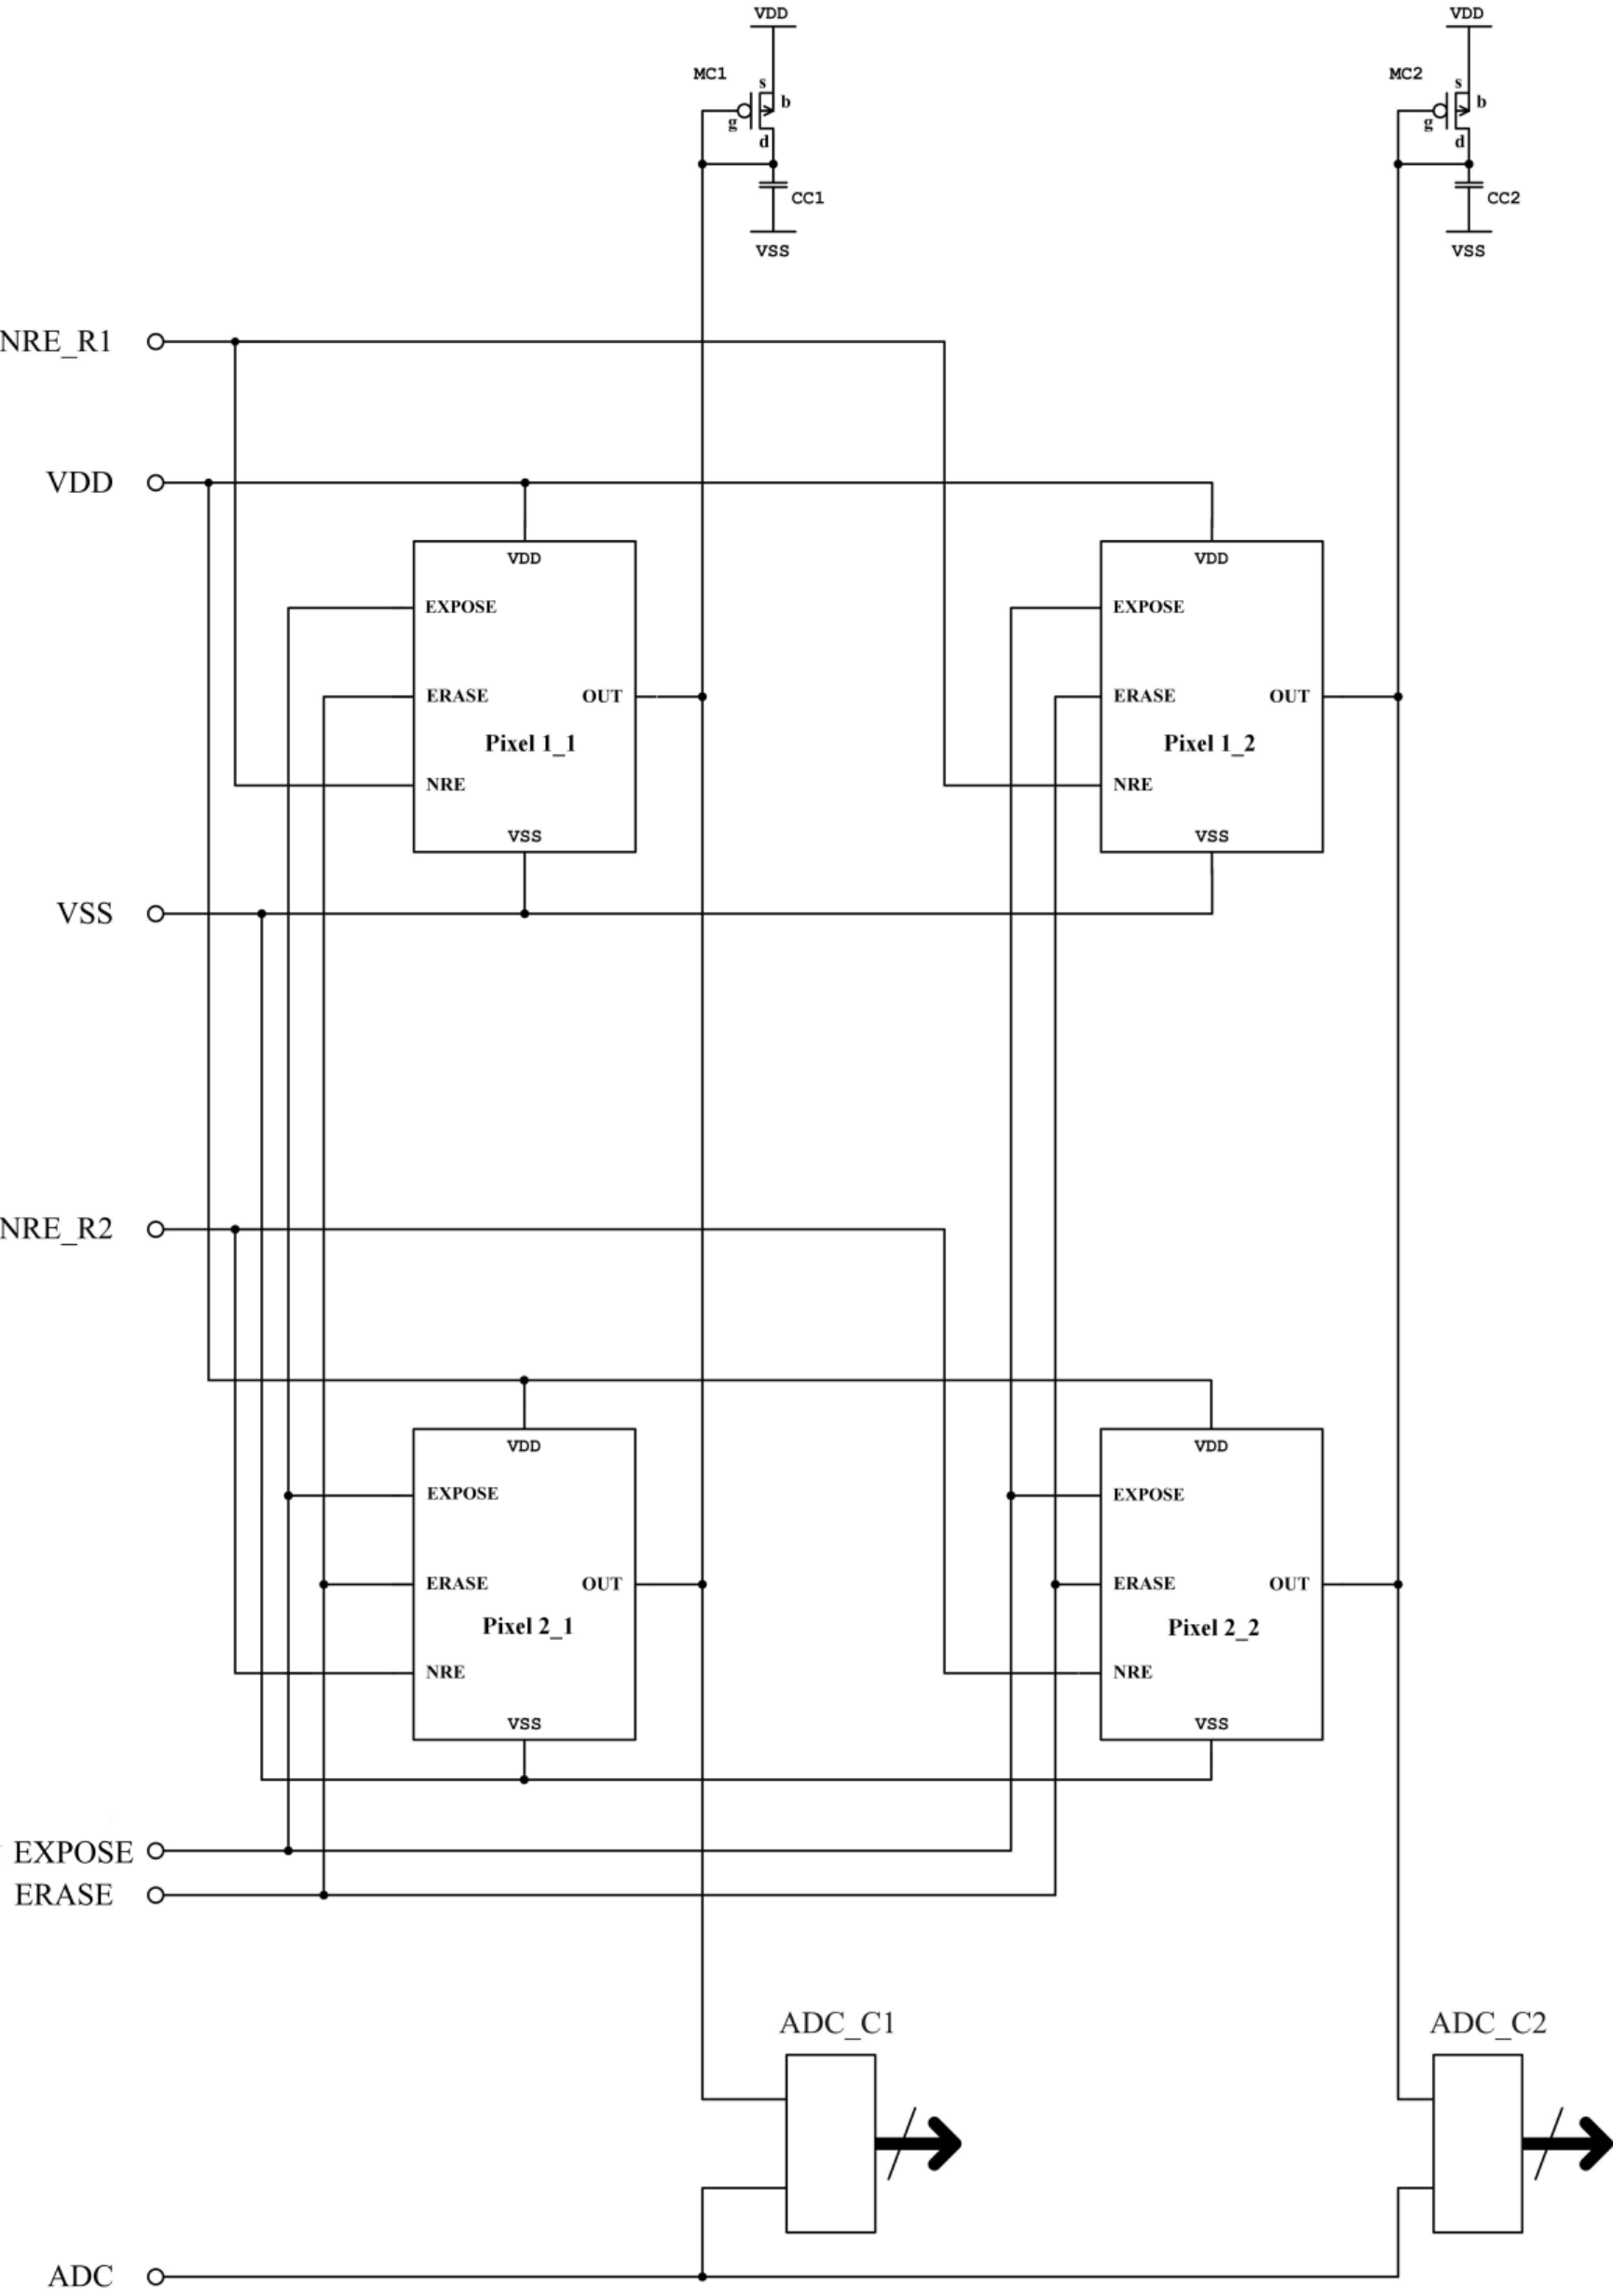
\includegraphics[width=0.8\textwidth]{graphs/analogCircuit.png}
    \caption{Analog circuit schematic.}
    \label{fig:analogCircuit}
\end{figure}

\begin{figure}
    \centering
    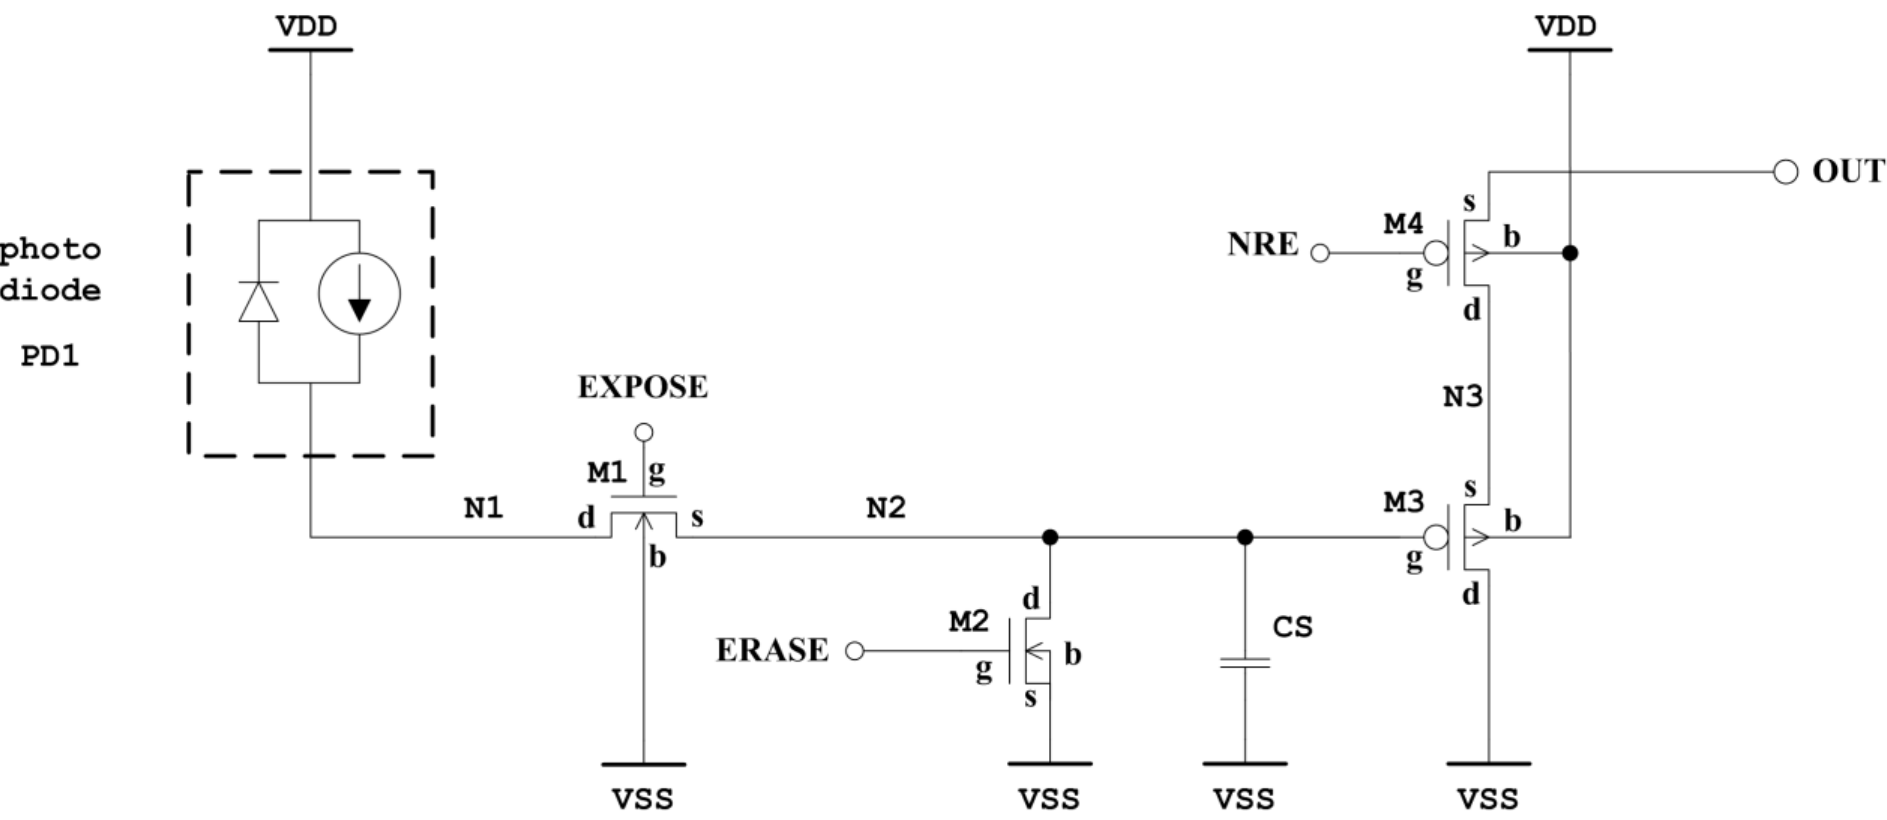
\includegraphics[width=\textwidth]{graphs/pixelCircuit.png}
    \caption{Pixel cicuit schematic.}
    \label{fig:pixelCircuit}
\end{figure}

In detail, the analog circuit consists of 4 pixels in a 2x2 array. Each pixel in the same row shares the same NRE (Not-REad) input which means they are sending data to the ADC at the same time. Each pixel in the same column share the same active load and readout wire, which means they need to send data to the ADC at different times.

\subsubsection{Detailed decription of pixel circuit}

Schematics for the pixel circuit is given in figure \ref{fig:pixelCircuit}. It consists of a photo diode PD1, three switch transistors M1, M2 and M4, one buffer transistor M3 and a charge storage capacitor $C_S$. The photo diode is modeled by a diode and an ideal current source in parallel. The current source outputs a current $I_D$ that is proportional to the illumination intensity on that particular pixel. This current is used to charge the transistor $C_S$. Ideally, we want that all of $I_D$ flows through M1 and into CS when EXPOSE is high and all of $I_D$ flows back through the diode in the photo diode model when EXPOSE is low.

\subsubsection{Dimensions for switch transistors}
\label{sec:switch_dimensions}
The transistors M1, M2 and M4 all function as switches, where a digital gate input decides whether the transistor should act as a short-circuit between drain and source, or as an open circuit. Since these transistors simply should have two possible states, it is key that the leakage current is minimized. This is particularly important for M1 and M2 to ensure that the voltage over $C_s$ is as constant as possible during readout. In \emph{Analog Circuit Design} by Tony Chan Carusone, one can read in section 1.4.1 that the subthreshold leakage current is given by

\begin{equation}
    \label{eq:leakage}
    I_{off} = (n-1) \mu_n C_{ox} \left( \frac{W}{L} \right) \left( \frac{kT}{q} \right)^2 \exp{(-qV_t / nkT)}.
\end{equation}

In order to minimize this leakage current, $\frac{W}{L}$ need to be as small as possible, meaning the smallest possible width $W$ and the largest possible length $L$ is desired. The technology used will limit the possible width and length of the transistor, thus $W$ and $L$ can be chosen accordingly.

\subsubsection{Value for $C_s$}

To choose a suitable value for $C_s$ spice simulations can be used. To know what values are the best we will look at the four corner cases for exposure time and light conditions. The corner cases will be denoted exposure-light, so for example max-min is maximum exposure time and minimum light. For each corner we will do a transient simulation. That means we will look at a graph that shows the voltage over $C_s$ as a function of time. In each light-exposure corner, the resulting voltage value that we are interested in is the voltage over $C_s$ at the end of the exposure. There are many possible approaches to how these corners should be tuned, and the one that we will apply is the following:

\begin{itemize}
    \item Max-max corner should make $C_s$ fully charged.
    \item Min-min corner should leave $C_s$ uncharged.
    \item Min-max and max-min corners should make $C_s$ half full charged.
\end{itemize}

The reason for why we want the corners to be like that is beyond the scope of this report.

\subsubsection{Values for M3 and active load}

\subsection{Digital camera controller}

\subsubsection{Finite state machine}

\subsubsection{Output timing}

\subsubsection{Module interface}

\begin{figure}
    \centering
    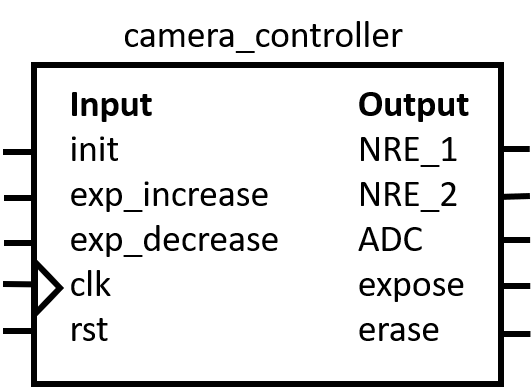
\includegraphics[width=0.7\textwidth]{graphs/camera_controller_pinout.png}
    \caption{Overview of input and output pins as well as internal regististers for the camera controller module.}
\end{figure}
